
本章主要讲解动态规划的几种基础 \textbf{ 优化 } 方法。

\subsection{二进制优化解多重背包}

\begin{NOTE}{ 例题 [经典问题 - 多重背包](/dp/backpack/#_3)}{}
题目大意:有 $n$ 种物品,每种物品有 $a_i$ 件,购买一件这种物品的费用为 $c_i$,价值为 $v_i$。有一个容量为 $t$ 的背包,现在让你找到最优的一种方案,使得装入背包的物品的总价值最大。
\end{NOTE}


考虑常规的动规方式,定义 $f_{i,j}$ 为当前考虑到第 $i$ 个物品,背包容量为 $j$ 所能获得的最大价值。

状态转移方程为, $f_{i,j}=\max\{f_{i-1,j},f_{i-1,j-c_i}+v_i\}$。

对于 \textbf{ 每件 } 物品,都要这样循环一次,时间复杂度为 $t\times \sum_{i=1}^n a_i$,某些时候可能不可接受,需要优化。

考虑这样一种情况,如果我们有 $17$ 个硬币,要去买 $1$ 到 $17$ 元钱的物品,只需将这些硬币打包成 $1,2,4,8$ 和 $2$ 这样的几包。前面的 $4$ 包能保证覆盖 $1$ 到 $15$ 所有的情况,最后一包在之前的基础上再加上一个值,能保证实现支付的时候取整包,肯定能保证支付。这就是二进制优化的原理和基本思想。

用上述的方法,就可以把 $k$ 件相同的物品看作是 $O(log_2 k)$ 件物品了。优化后

代码实现:

\begin{cppcode}
for (int i = 1; i <= n; i++) {
  scanf("%d", a + i);
  tot += c[i] * a[i];
  for (int j = 1; j <= a[i]; j *= 2)
    if (a[i] >= j) a[i] -= j, v[++cur] = c[i] * j;
  if (a[i]) v[++cur] = c[i] * a[i];
}
for (int i = 1; i <= cur; i++)
  for (int j = m; j >= v[i]; j--)
    if (f[j - v[i]]) f[j] = true;
\end{cppcode}

\subsection{几道练习题}

\href{http://acm.hdu.edu.cn/showproblem.php?pid=2844}{HDU 2844 Coins}

\subsection{单调队列 \& 单调栈优化}

学习本节前,请务必先学习 \href{/ds/monotonous-queue/}{单调队列}。

\begin{NOTE}{ 例题 [CF372C Watching Fireworks is Fun](http://codeforces.com/problemset/problem/372/C)}{}
题目大意:城镇中有 $n$ 个位置,有 $m$ 个烟花要放。第 $i$ 个烟花放出的时间记为 $t_i$,放出的位置记为 $a_i$。如果烟花放出的时候,你处在位置 $x$,那么你将收获 $b_i-|a_i-x|$ 点快乐值。初始你可在任意位置,你每个单位时间可以移动不大于 $d$ 个单位距离。现在你需要最大化你能获得的快乐值。
\end{NOTE}


设 $f_{i,j}$ 表示在放第 $i$ 个烟花时,你的位置在 $j$ 所能获得的最大快乐值。

写出 \textbf{ 状态转移方程 } :$f_{i,j}=\max\{f_{i-1,k}+b_i-|a_i-j|\}$

这里的 $k$ 是有范围的,$j-(t_{i+1}-t_i)\times d\le k\le j+(t_{i+1}-t_i)\times d$。

我们尝试将状态转移方程进行变形:

由于 $\max$ 里出现了一个确定的常量 $b_i$,我们可以将它提到外面去。

$f_{i,j}=\max\{f_{i-1,k}+b_i+|a_i-j|\}=\max\{f_{i-1,k}-|a_i-j|\}+b_i$

如果确定了 $i$ 和 $j$ 的值,那么 $|a_i-j|$ 的值也是确定的,也可以将这一部分提到外面去。

最后,式子变成了这个样子:$f_{i,j}=\max\{f_{i-1,k}-|a_i-j|\}+b_i=\max\{f_{i-1,k}\}-|a_i-j|+b_i$

看到这一熟悉的形式,我们想到了什么?\textbf{ 单调队列优化 }。由于最终式子中的 $\max$ 只和上一状态中连续的一段的最大值有关,所以我们在计算一个新的 $i$ 的状态值时候只需将原来的 $f_{i-1}$ 构造成一个单调队列,并维护单调队列,使得其能在均摊 $O(1)$ 的时间复杂度内计算出 $\max\{f_{i-1,k}\}$ 的值,从而根据公式计算出 $f_{i,j}$ 的值。

总的时间复杂度为 $O(n\times m)$。

讲完了,让我们归纳一下单调队列优化动态规划问题的基本形态:当前状态的所有值可以从上一个状态的某个连续的段的值得到,要对这个连续的段进行 RMQ 操作,相邻状态的段的左右区间满足非降的关系。

\subsubsection{几道练习题:}

\href{https://www.luogu.org/problemnew/show/P1886}{洛谷 P1886 滑动窗口}

\href{https://www.luogu.org/problemnew/show/P2254}{洛谷 P2254 \textbackslash{}[NOI2005\textbackslash{}] 瑰丽华尔兹}

\href{https://www.luogu.org/problemnew/show/P2569}{洛谷 P2569 \textbackslash{}[SCOI2010\textbackslash{}] 股票交易}

\subsection{斜率优化}

\begin{NOTE}{ 例题 [洛谷 P3195 \[HNOI2008\] 玩具装箱 TOY](https://www.luogu.org/problemnew/show/P3195)}{}
令 $f_i$ 表示前 $i$ 个物品,随意分组装在任意多个容器里所能得到的最小费用。
\end{NOTE}


写出 \textbf{ 状态转移方程 } :$f_i=max\{f_j+(pre_i-pre_i+i-j-1-L)^2\}$ ,其中 $pre_i$ 表示前 $i$ 个数的前缀和。

换元试图简化状态转移方程式: 令 $s_i=pre_i+i,L'=L+1$,则 $f_i=f_j+(s_i-s_j-L')^2$,展开,移项得

$f_i=f_j+(s_i-s_j-L')^2$

$f_i+2\times s_i\times (s_j+L')=f_j+s_i^2+(s_j+L')^2$

我们观察到,式子的右端的所有项都只和 $i$ 有关或只和 $j$ 有关,式子左端的第一项是我们要求的目标值,式子左端的其余项都同时和 $i$ 和 $j$ 有关。我们将这个式子看作一条直线的函数解析式,形如 $b+k\times x=y$ ,和上式一一对应。我们发现如果我们要最小化 $f_i$ ,也就是说要最小化这个直线的截距,而对于每个确定的 $i$,这个直线的斜率 $s_i$ 都是确定的。

\begin{figure}[h]
\centering
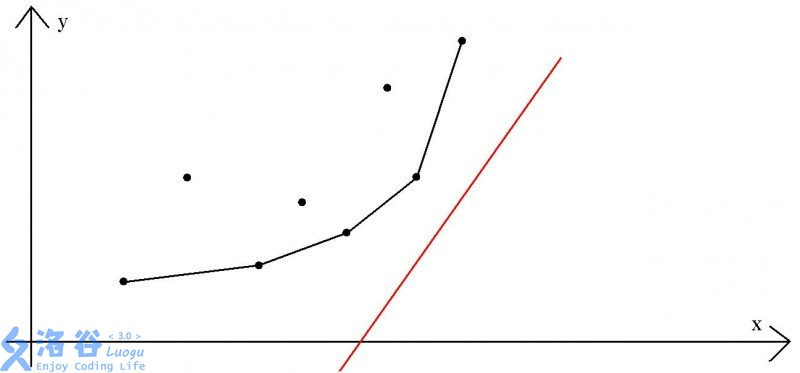
\includegraphics[width=0.5\textwidth]{images/optimization.png} 

\end{figure}

如图,我们将这个斜率固定的直线从下往上平移,直到有一个点在这条直线上,然后将新的点加入点集,这样肯定能保证所有的直线的斜率都是单调递升的(因为如果新的直线斜率小于斜率最大的直线,那么其一定不成被选择成为新的决策),所以我们相当于维护了一个下凸包。(如果求的是 $\max$ 那么就要维护一个 \textbf{ 上凸包 } 。这种东西要具体情况具体分析,如果直线的斜率不满足单调性,那就要维护整个凸包 / 二分等奇技淫巧。)

可以用单调队列维护下凸包。

\subsubsection{几道练习题:}

\href{https://www.luogu.org/problemnew/show/P4072}{洛谷 P4072 \textbackslash{}[SDOI2016\textbackslash{}] 征途}

\href{https://www.luogu.org/problemnew/show/P2120}{洛谷 P2120 \textbackslash{}[ZJOI2007\textbackslash{}] 仓库建设}

\href{https://www.luogu.org/problemnew/show/P3628}{洛谷 P3628 \textbackslash{}[APIO2010\textbackslash{}] 特别行动队}

\href{https://www.lydsy.com/JudgeOnline/problem.php?id=4709}{bzoj 4709 \textbackslash{}[Jsoi2011\textbackslash{}] 柠檬}

\href{http://codeforces.com/problemset/problem/311/B}{CF311B Cats Transport}

\href{https://www.luogu.org/problemnew/show/P4027}{洛谷 P4027 \textbackslash{}[NOI2007\textbackslash{}] 货币兑换}

\subsection{四边形不等式优化}

\begin{NOTE}{ 例题 [洛谷 P1880 \[NOI1995\] 石子合并](https://www.luogu.org/problemnew/show/P1880)}{}
题目大意:在一个环上有 $n$ 个数,进行 $n-1$ 次合并操作,每次操作将相邻的两堆合并成一堆,能获得新的一堆中的石子数量的和的得分。你需要最大化你的得分。
\end{NOTE}


我们首先 \textbf{ 破环成链 } ,然后进行动态规划。设 $f_{i,j}$ 表示从位置 $i$ 合并到位置 $j$ 所能得到的最大得分, $sum_i$ 为前 $i$ 堆石子数的前缀和。

写出 \textbf{ 状态转移方程 } : $f_{i,j}=\max\{f_{i,k}+f_{k+1,j}+(sum_j-sum_i)\}(i\le k\le j)$

考虑常规的转移方法,枚举 $i$、$j$ 和 $k$,时间复杂度为 $O(n^3)$。

\subsubsection{什么是四边形不等式?}

对于 $a<b\le c<d$,如果有$f_{a,c}+f_{b,d}\le f_{b,c}+f_{a,d}$,则称该数组满足四边形不等式,可以用通俗的方法表述为 “交叉小于包含”。

两个定理:

\begin{enumerate}
\item 四边形不等式能优化的状态转移方程能表示为 $f_{i,j}=\max\{f_{i,k}+f_{k+1,j}+cost(i,j)\}(i\le k\le j)$。如果 $cost$ 函数同时满足单调性和四边形不等式,那么数组 $f$ 也满足四边形不等式。
\item 定义 $idx_{i,j}$ 为在转移 $f_{i,j}$ 的过程中在 $k=idx_{i,j}$ 时取得最小值,那么有如下定理:
如果 $f$ 数组满足四边形不等式,那么 $idx$ 函数满足单调性,即有 $idx_{i,j}\le idx_{i,j+1}\le idx_{i+1,j+1}$ 。
\end{enumerate}

证明会和题目解法一起 $qwq$ 

\subsubsection{回到题目}

第一步:证明 $cost$ 满足四边形不等式

要证明,对于所有满足 $i<i+1\le j<j+1$ 的 $i,j$ , 均有 $cost_{i,j}+cost_{i+1,j+1}\le cost_{i+1,j}+cost_{i,j+1}$。

移项得 $cost_{i,j}-cost_{i+1,j}\le cost_{i,j+1}-cost_{i+1,j+1}$

设 $F(j)=cost_{i,j}-cost{i+1,j}$ ,如果要使这个四边形不等式成立,那么就要证明 $F(j)$ 单调非降。

在本题中, $F(j)=(sum_j-sum_{i-1})-(sum_j-sum_i)=sum_i-sum_{i-1}=a_i$ ,与 $j$ 无关,自然一定满足四边形不等式。

证毕。

第二步:证明 $f$ 满足四边形不等式

同样的,应有如下结论:对于所有满足 $i<i+1\le j<j+1$ 的 $i,j$ , 均有 $f_{i,j}+f_{i+1,j+1}\le f_{i+1,j}+f_{i,j+1}$

我们假设 $x=idx_{i+1,j},y=idx_{i,j+1}$。不妨设 $x<=y$。

将 $x,y$ 带入得,$f_{i,j}+f_{i+1,j+1}=f_{i,x}+f_{x+1,j}+cost_{i,j}+f_{i+1,y}+f_{y+1,j+1}+cost_{i+1,j+1}$

由于上一步已经证明出了$cost$满足四边形不等式,而该不等式的左边在上式出现过,将其替换得

$$
\begin{aligned}
&&f_{i,\,x}+f_{x+1,\,j}+cost_{i,\,j}+f_{i+1,\,y}+f_{y+1,\,j+1}+cost_{i+1,\,j+1}\\
&\le&f_{i,\,x}+f_{x+1,\,j+1}+cost_{i,\,j+1}+f_{i+1,\,y}+f_{y+1,\,j}+cost_{i+1,\,j}\\
\end{aligned}
$$

消去公共项可得 $f_{i,j}+f_{i+1,j+1}\le f_{i+1,j}+f_{i,j+1}$

证毕。

第三步:证明决策的单调性

现在我们已经证明了 $cost$ 和 $f$ 满足四边形不等式,要证明决策的单调性以证明优化的正确性。

即证 $idx_{i,j-1}\le idx_{i,j}\le idx_{i+1,j}$

我们只证明式子的前半部分,后半部分可以有类似的方法推出。

设 $y=idx_{i,j-1},x\le y$ ,因为 $x+1\le y+1\le j-1<j$,由四边形不等式可得,

$f_{x+1,j-1}+f_{y+1,j}\le f_{y+1,j-1}+f_{x+1,j}$

由于我们是令 $y=idx_{i,j-1},x\le y$ 时 $f_{i,j-1}$ 取得最小值,那么 $f_{i,j-1}(idx_{i,j-1}=x)$ 一定大于等于 $f_{i,j-1}(idx_{i,j-1}=y)$ ,所以对于 $f_{i,j-1}$ 可以取到最优值的 $y$ ,所有小于它的值,对于 $f_{i,j}$ 来说,都没有 $y$ 优,所以最优决策一定不是小于 $y$ 的,那么一定有 

$idx_{i,j-1}\le idx_{i,j}$ 

证毕。

\subsubsection{说了这么多,怎么进行状态转移呢?}

给出核心代码:

\begin{cppcode}
for (int i = n; i >= 1; i--) {
  for (int j = i + 1; j <= n; j++) {
    f[i][j] = inf;
    for (int k = s[i][j - 1]; k <= s[i + 1][j]; k++) {
      if (f[i][j] < f[i][k] + f[k + 1][j] + sum[j] - sum[i - 1]) {
        f[i][j] = f[i][k] + f[k + 1][j] + sum[j] - sum[i - 1];
        idx[i][j] = k;
      }
    }
  }
}
\end{cppcode}

注意:由于在计算 $f_{i,j}$ 的时候需要知道 $idx_{i,j-1}$ 和 $idx_{i+1,j}$ 的值,所以 $i$ 的循环逆序。

\subsubsection{时间复杂度证明}

计算 $f_{i,j}$ 时,我们要循环 $idx_{i+1,j}-idx_{i,j-1}$ 次,那么一共加起来会循环多少次呢?

因为 $\sum_{i=1}^{n-1}(idx_{i+1,i+1}-idx_{i,i})=idx_{n,n}-idx_{1,1}$ 很显然和 $n$ 同阶,那么它的 $n$ 倍就和 $n^2$ 同阶,时间复杂度是 $O(n^2)$。

\subsubsection{一道练习题:}

\href{https://www.luogu.org/problemnew/show/P4767}{洛谷 P4767 \textbackslash{}[IOI2000\textbackslash{}] 邮局}

\subsubsection{参考资料}

\href{https://blog.csdn.net/noiau/article/details/72514812}{NOIAu 的 CSDN 博客}
